\documentclass[tikz,border=3mm]{standalone}
\usetikzlibrary{shapes.geometric}

\begin{document}
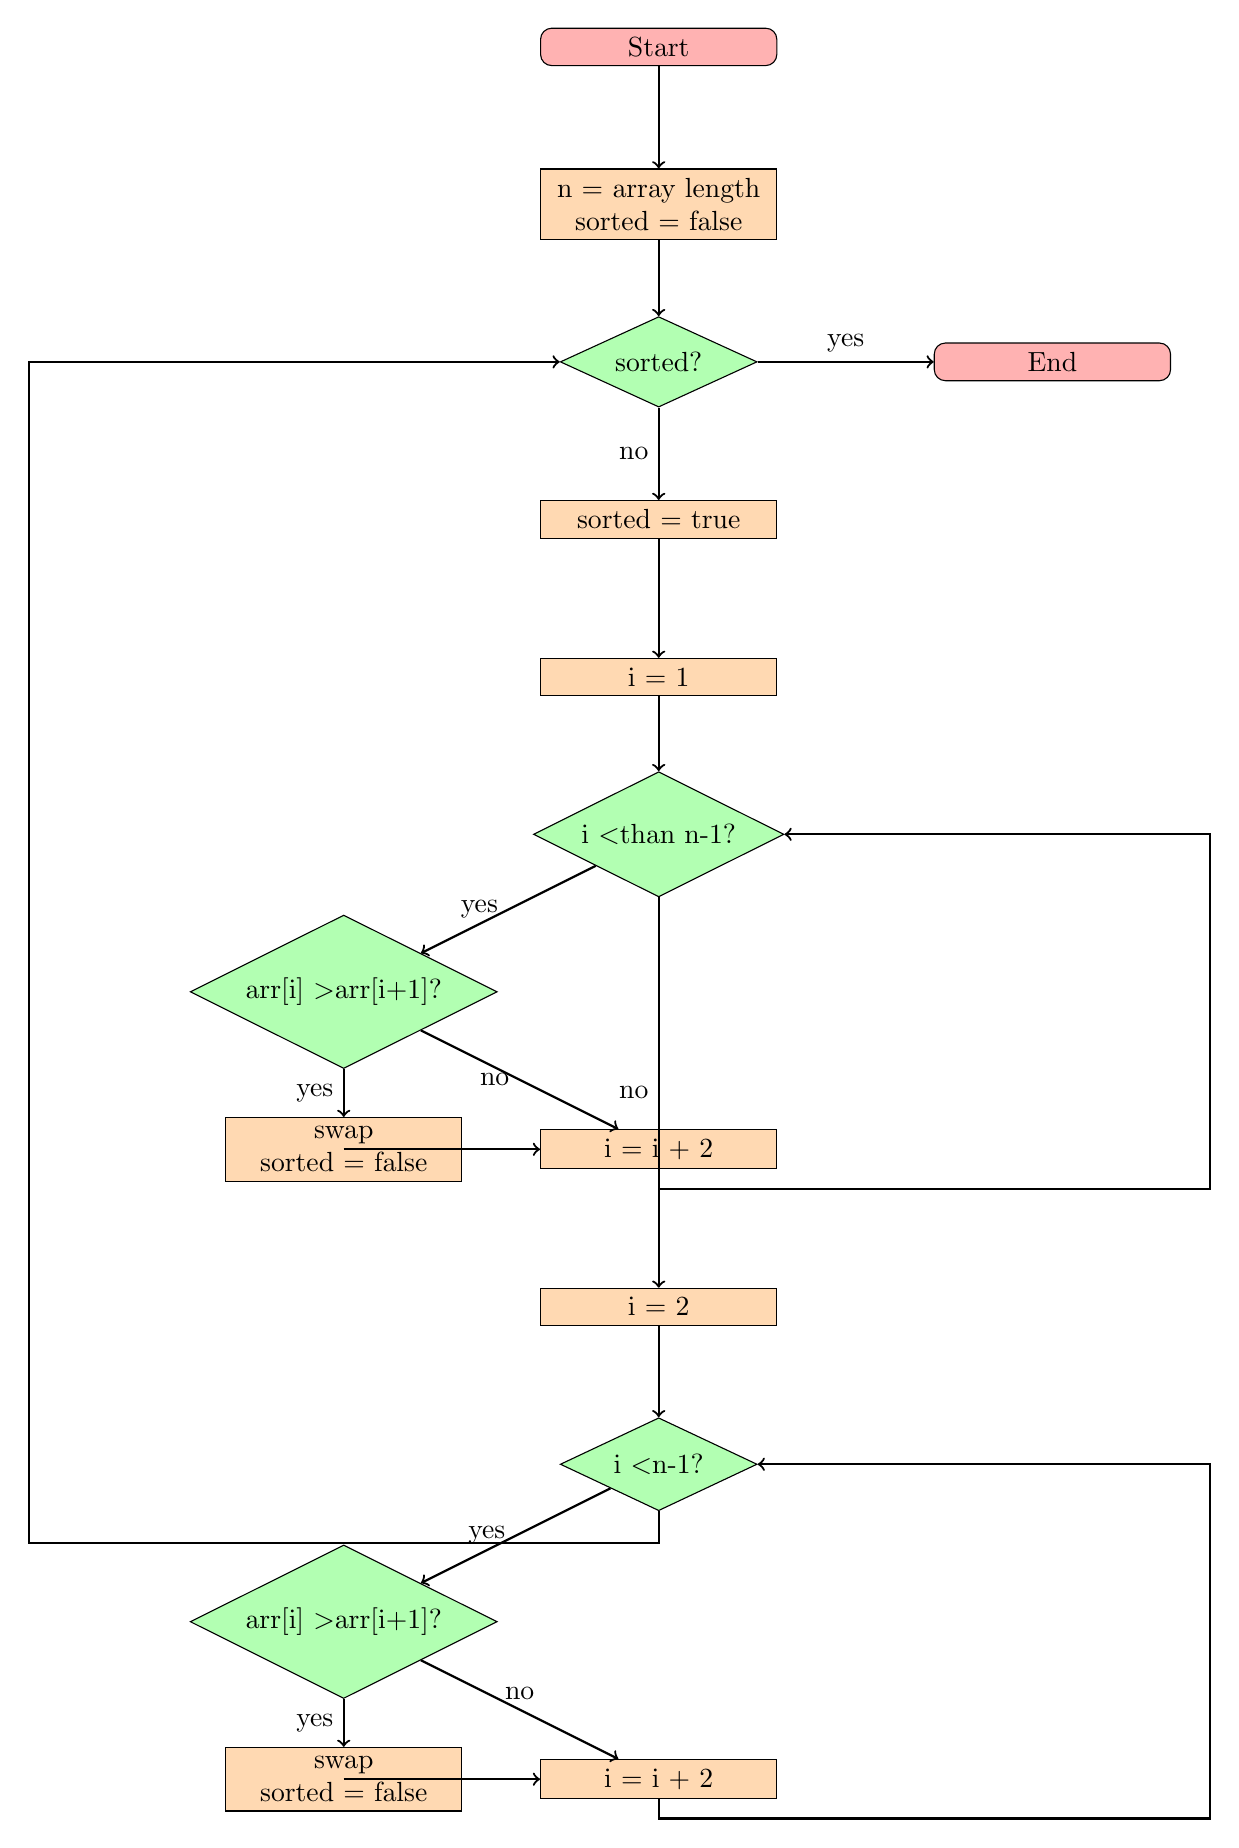
\begin{tikzpicture}[
    every node/.style={align=center}
]

% Блоки с цветами
\node[draw=black, fill=red!30, rectangle, rounded corners, minimum width=3cm] (start) at (0,0) {Start};
\node[draw=black, fill=orange!30, rectangle, minimum width=3cm] (init) at (0,-2) {n = array length\\sorted = false};
\node[draw=black, fill=green!30, diamond, minimum width=2.5cm, aspect=2] (check) at (0,-4) {sorted?};
\node[draw=black, fill=orange!30, rectangle, minimum width=3cm] (set) at (0,-6) {sorted = true};
\node[draw=black, fill=orange!30, rectangle, minimum width=3cm] (odd) at (0,-8) {i = 1};
\node[draw=black, fill=green!30, diamond, minimum width=2.5cm, aspect=2] (odd_cond) at (0,-10) {i \textless than n-1?};
\node[draw=black, fill=green!30, diamond, minimum width=2.5cm, aspect=2] (odd_comp) at (-4,-12) {arr[i] \textgreater arr[i+1]?};
\node[draw=black, fill=orange!30, rectangle, minimum width=3cm] (odd_swap) at (-4,-14) {swap\\sorted = false};
\node[draw=black, fill=orange!30, rectangle, minimum width=3cm] (odd_inc) at (0,-14) {i = i + 2};
\node[draw=black, fill=orange!30, rectangle, minimum width=3cm] (even) at (0,-16) {i = 2};
\node[draw=black, fill=green!30, diamond, minimum width=2.5cm, aspect=2] (even_cond) at (0,-18) {i \textless n-1?};
\node[draw=black, fill=green!30, diamond, minimum width=2.5cm, aspect=2] (even_comp) at (-4,-20) {arr[i] \textgreater arr[i+1]?};
\node[draw=black, fill=orange!30, rectangle, minimum width=3cm] (even_swap) at (-4,-22) {swap\\sorted = false};
\node[draw=black, fill=orange!30, rectangle, minimum width=3cm] (even_inc) at (0,-22) {i = i + 2};
\node[draw=black, fill=red!30, rectangle, rounded corners, minimum width=3cm] (end) at (5,-4) {End};

% Стрелки
\draw[->, thick] (start) -- (init);
\draw[->, thick] (init) -- (check);
\draw[->, thick] (check) -- node[left] {no} (set);
\draw[->, thick] (set) -- (odd);
\draw[->, thick] (odd) -- (odd_cond);
\draw[->, thick] (odd_cond) -- node[left] {yes} (odd_comp);
\draw[->, thick] (odd_comp) -- node[left] {yes} (odd_swap);
\draw[->, thick] (odd_swap) |- (odd_inc);
\draw[->, thick] (odd_comp) -- node[left] {no} (odd_inc);
\draw[->, thick] (odd_inc) -- ++(0,-0.5) -- ++(7,0) |- (odd_cond);
\draw[->, thick] (odd_cond) -- node[left] {no} (even);
\draw[->, thick] (even) -- (even_cond);
\draw[->, thick] (even_cond) -- node[left] {yes} (even_comp);
\draw[->, thick] (even_comp) -- node[left] {yes} (even_swap);
\draw[->, thick] (even_swap) |- (even_inc);
\draw[->, thick] (even_comp) -- node[above] {no} (even_inc);
\draw[->, thick] (even_inc) -- ++(0,-0.5) -- ++(7,0) |- (even_cond);
\draw[->, thick] (even_cond) -- ++(0,-1) -- ++(-8,0) |- (check);
\draw[->, thick] (check) -- node[above] {yes} (end);

\end{tikzpicture}
\end{document}